\newcommand{\usedspecs}[5]{
\begin{table}[h!]
\centering
\begin{tabular}{|c||c|} 
 \hline
 Interface & #1 \\
 \hline
 Sample rate & #2 \\ 
 \hline
 Data & #3 \\ 
 \hline
\end{tabular}
\caption{#4. Used technical specifications}
\label{table:#5_specs}
\end{table}
}

\chapter{Implementation}
\label{ch:Implementation}

\section{Hardware}
\label{sec:hardware}

Based on previous research a set of devices and sensors was selected (table \ref{table:hardware_peripherals}). The selection was done with a goal in mind: to utilize the maximum of the \emph{available space} on a human head and neck. Assuming that those surfaces will allow the recording of the vibrations and movements generated by the jaw bones and muscles. 

A Raspberry Pi 3 B+ (RPI) was used as the central processing unit (fig. \ref{image:prototype_overview}). It has a Bluetooth antenna as well as a variety of wired connectivity options to ease the build of this prototype. As discussed later in sec. \ref{sec:software} the RPI was used not only for the data collection but as well for the real-time data visualization. The RPI had some hardware limitations to read the raw data directly from some of the sensors. It was solved by using external microcontrollers (see \ref{subsub:bno}, \ref{subsub:emg} and \ref{subsub:tmic}).

All of the cables and attached devices were labeled accordingly to the side they have to be attached to, to maintain a reproducible setup between the participants of the user study.

\begin{figure}[h]
\centering
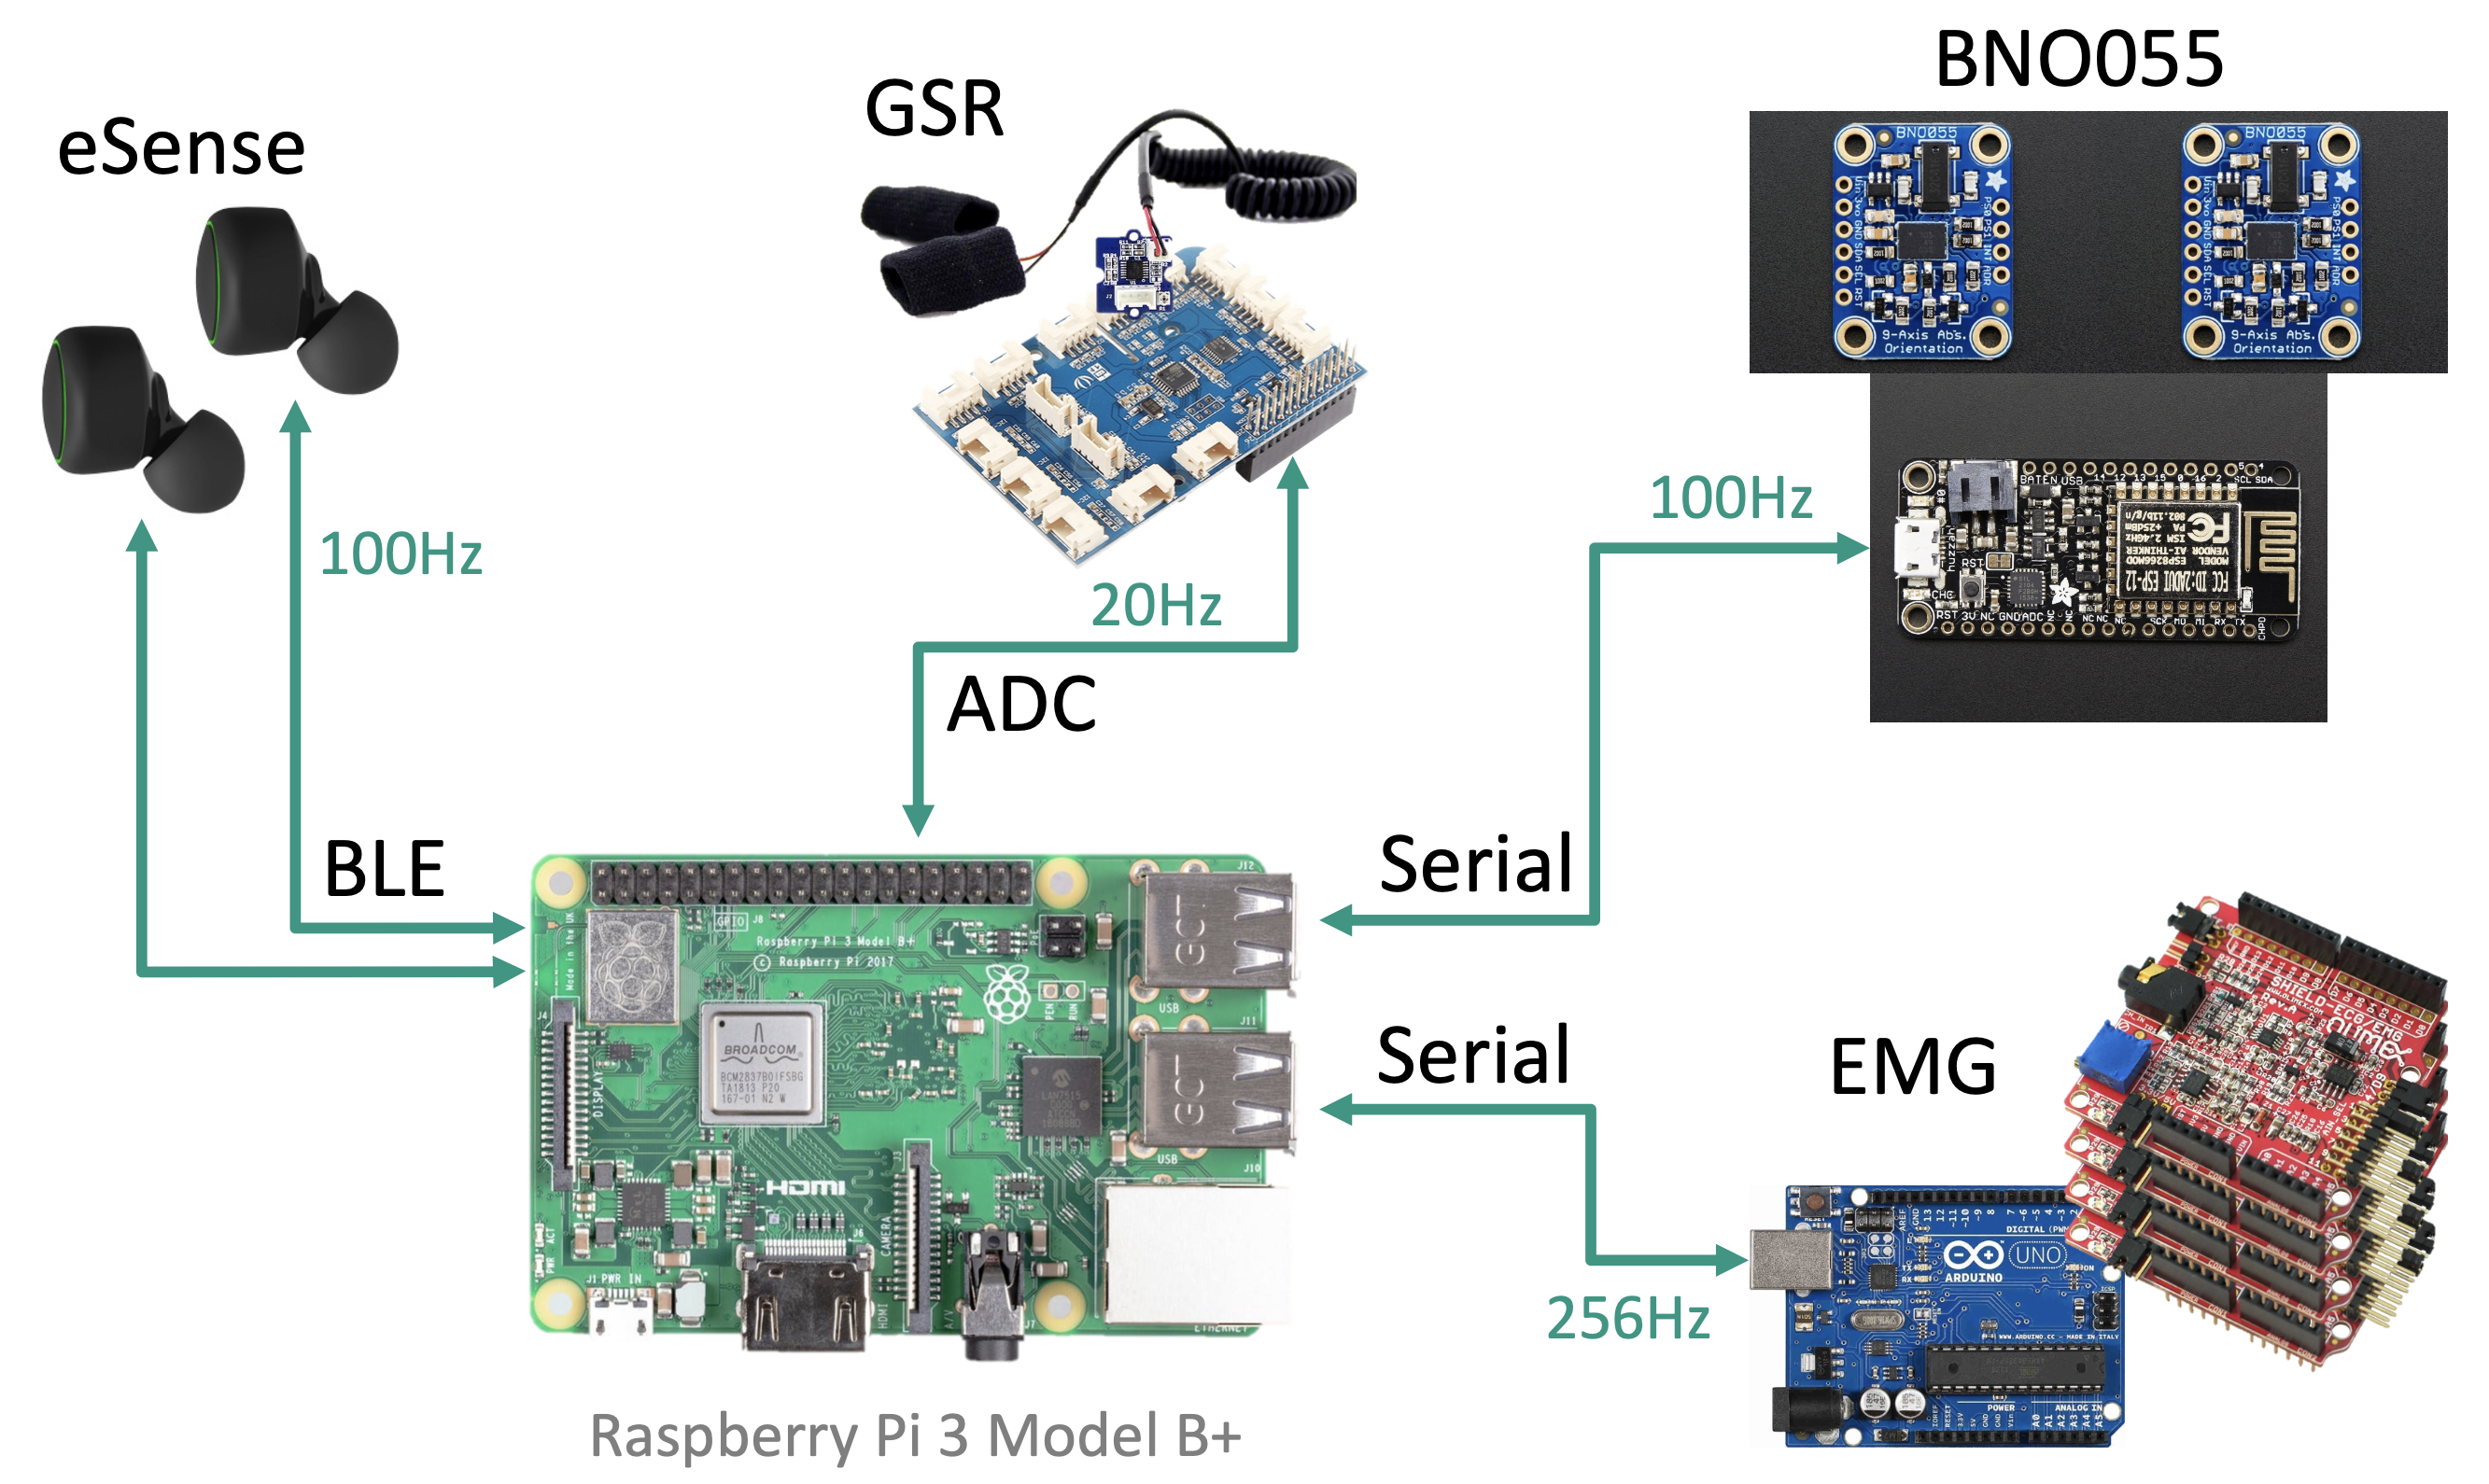
\includegraphics[width=0.8\textwidth]{src/media/hardware/overview.png}
\caption{Prototype Overview}
\label{image:prototype_overview}
\end{figure}

\subsection{Peripherals}

\begin{table}[!h]
\centering
\begin{tabular}{|>{\raggedright}m{0.25\linewidth}|>{\centering}m{0.1\linewidth}|m{0.3\linewidth}|m{0.25\linewidth}|} 
 \hline
 Device & Amount & Sensor & Area of contact \\ [0.5ex] 
 \hline\hline
 eSense earbuds \ref{subsub:esense} & 2 & 6 DOF IMU & In ear \\ 
 \hline
 Arduino BNO055 \ref{subsub:bno} & 2 & 9 DOF IMU & Back side of the jaw (secured with skin-friendly tape) \\ 
 \hline
 Olimex EMG-Shield & 4 & Electromyography (EMG) & Masseter and temporalis muscles \\ 
 \hline
 Throat microphone & 1 & Vibration sensor & Neck \\ 
 \hline
 Grove GSR & 1 & Galvanic skin response (GSR) & Index and middle finger \\ 
 \hline
\end{tabular}
\caption{Hardware peripherals}
\label{table:hardware_peripherals}
\end{table}

\subsubsection{eSense earables}
\label{subsub:esense}

\begin{figure}[h!]
\centering
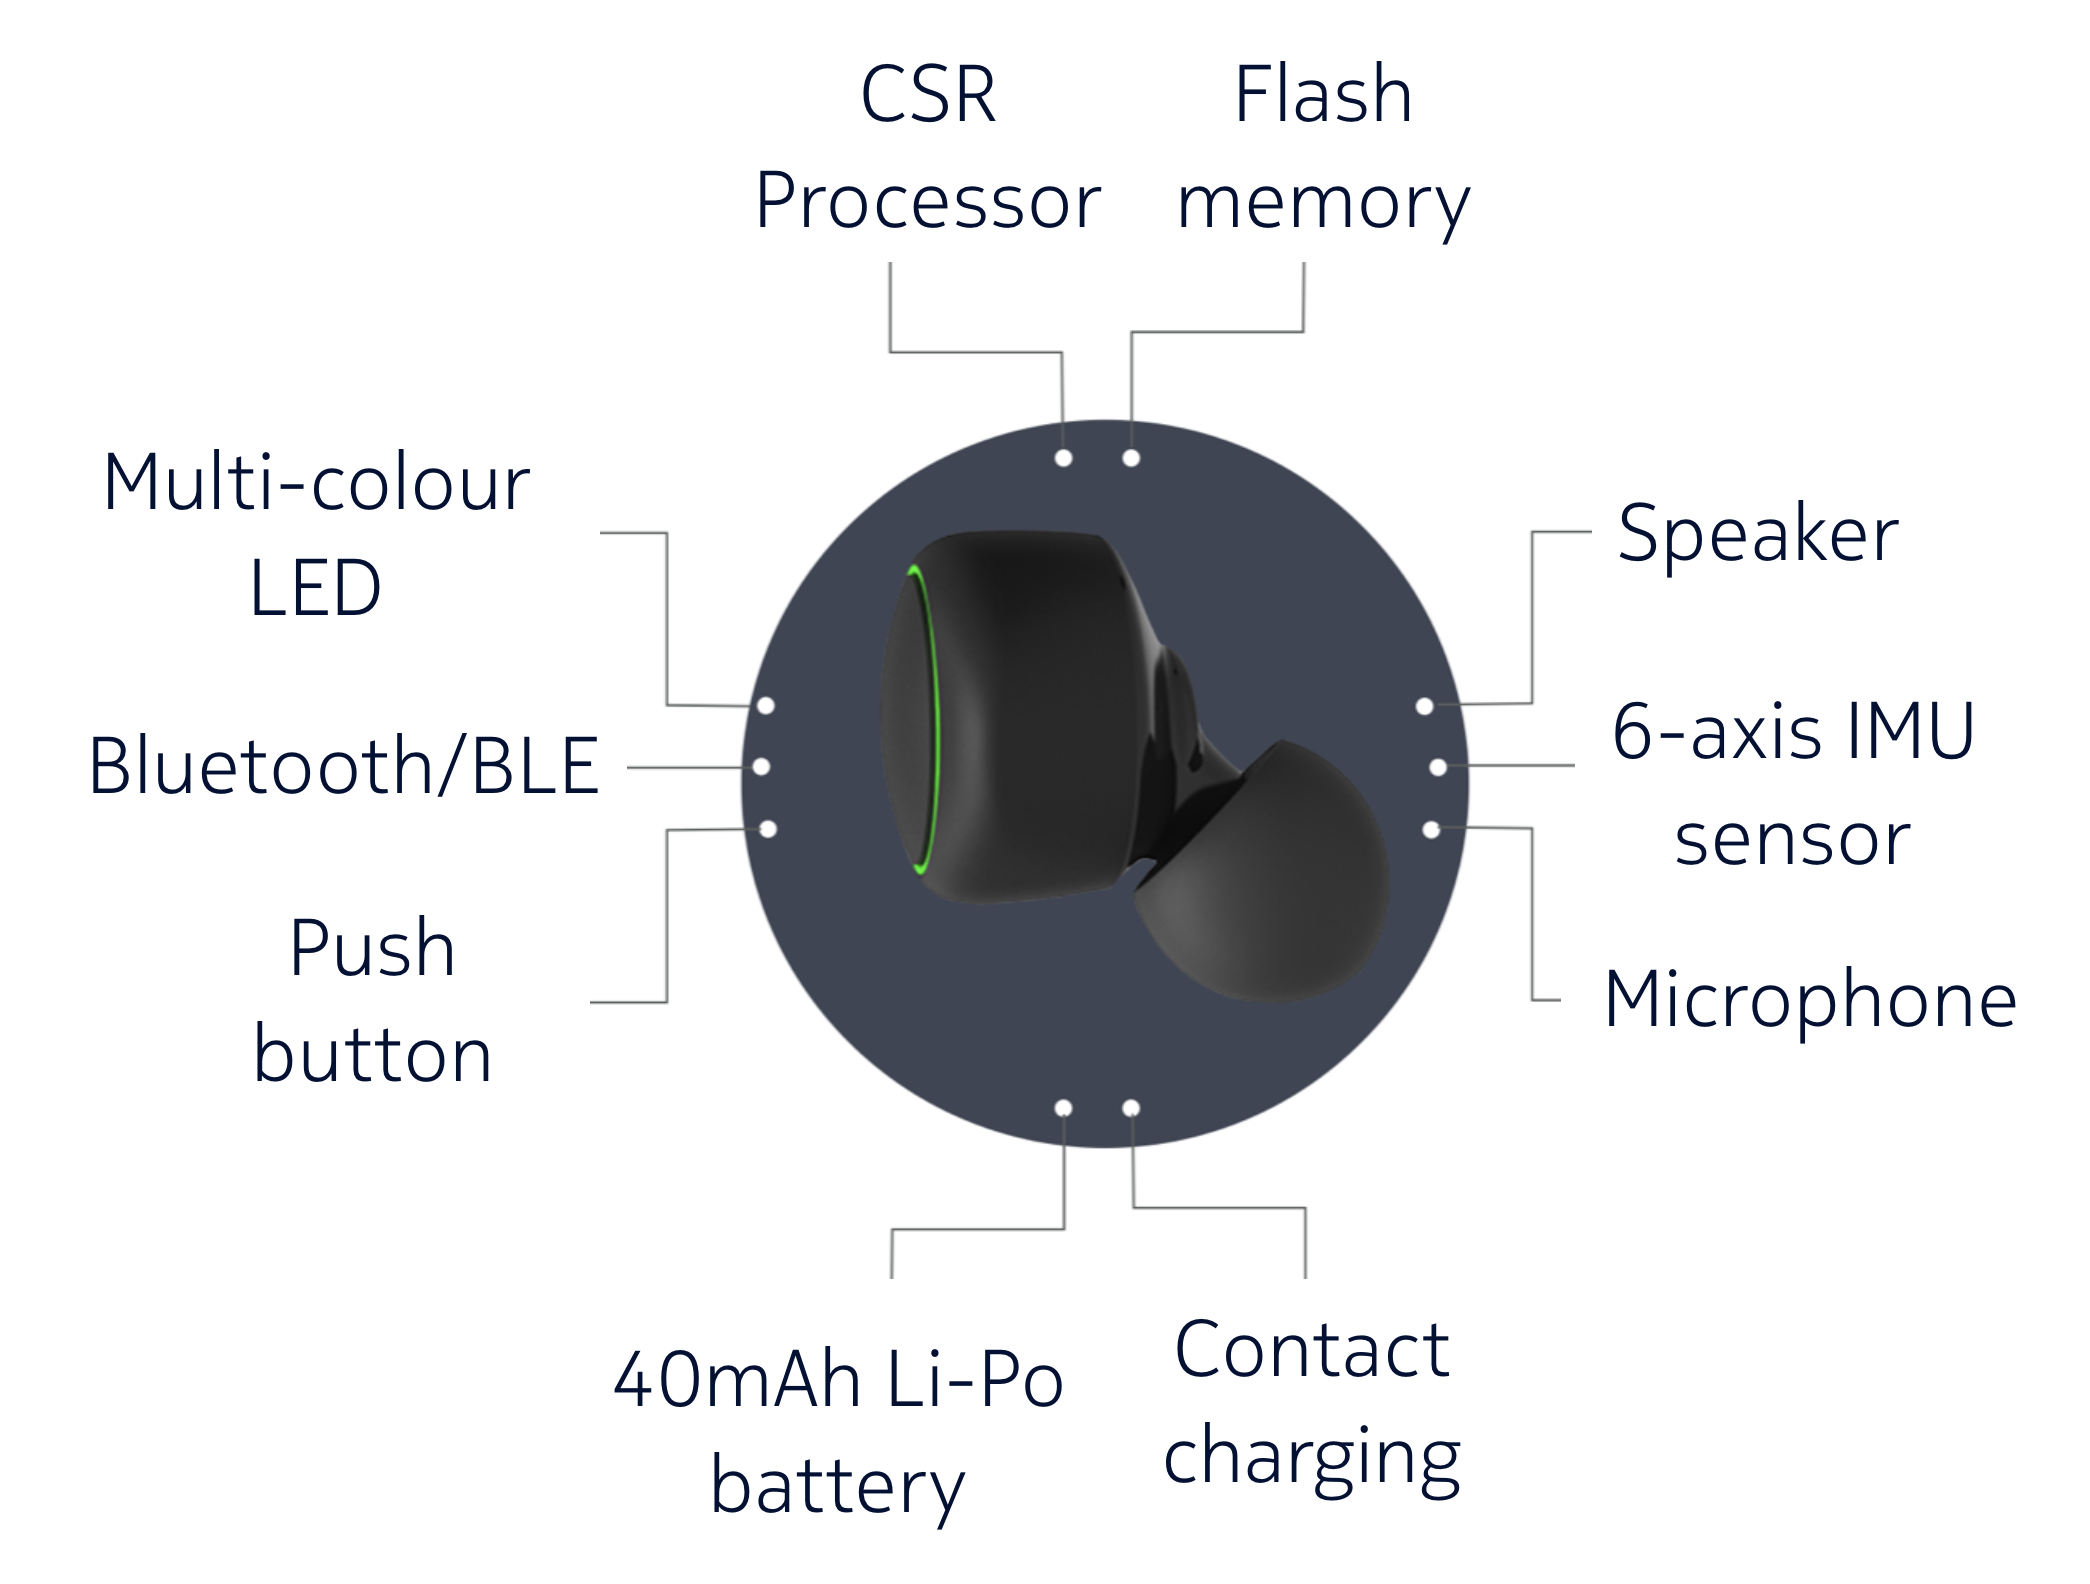
\includegraphics[width=0.5\textwidth]{src/media/hardware/esense.png}
\caption{eSense earable \cite{min2018exploring, kawsar2018earables}}
\label{image:esense}
\end{figure}

The eSense earables are a pair of true wireless earphones. The data we are interested in is the 6 DOF IMU located only in the left earpiece only. Because of this limitation, two left earpieces were used. Even though the left and right earpieces are not interchangeable, the participants in the user study didn't notice any difference in the fit in the right ear.

The default frequency of sending of the IMU data is set to 10Hz. In the case the audio playback is not being used, the frequency can be increased to up to 100Hz by changing the advertising and connection intervals (\cite{esense_ble_specification}), and still, have enough battery life for multiple user study recordings on a single battery charge. 

As a result, the IMU data from both earables was polled at 100Hz.

The connection was done directly with the RPI by using a python package called \texttt{bleak}. The incoming payload is a binary string that was decoded accordingly with the eSense specification \cite{esense_ble_specification}.

The IMU was kept at the default ranges of $\pm 4g$ for the accelerometer and $\pm 500deg/s$ for the gyroscope. No further transformations to other units were done.

\usedspecs{BLE}{100Hz}{Accelerometer \& gyroscope}{eSense earable}{esense}

\subsubsection{Arduino BNO055}
\label{subsub:bno}

\begin{figure}[h!]
\centering
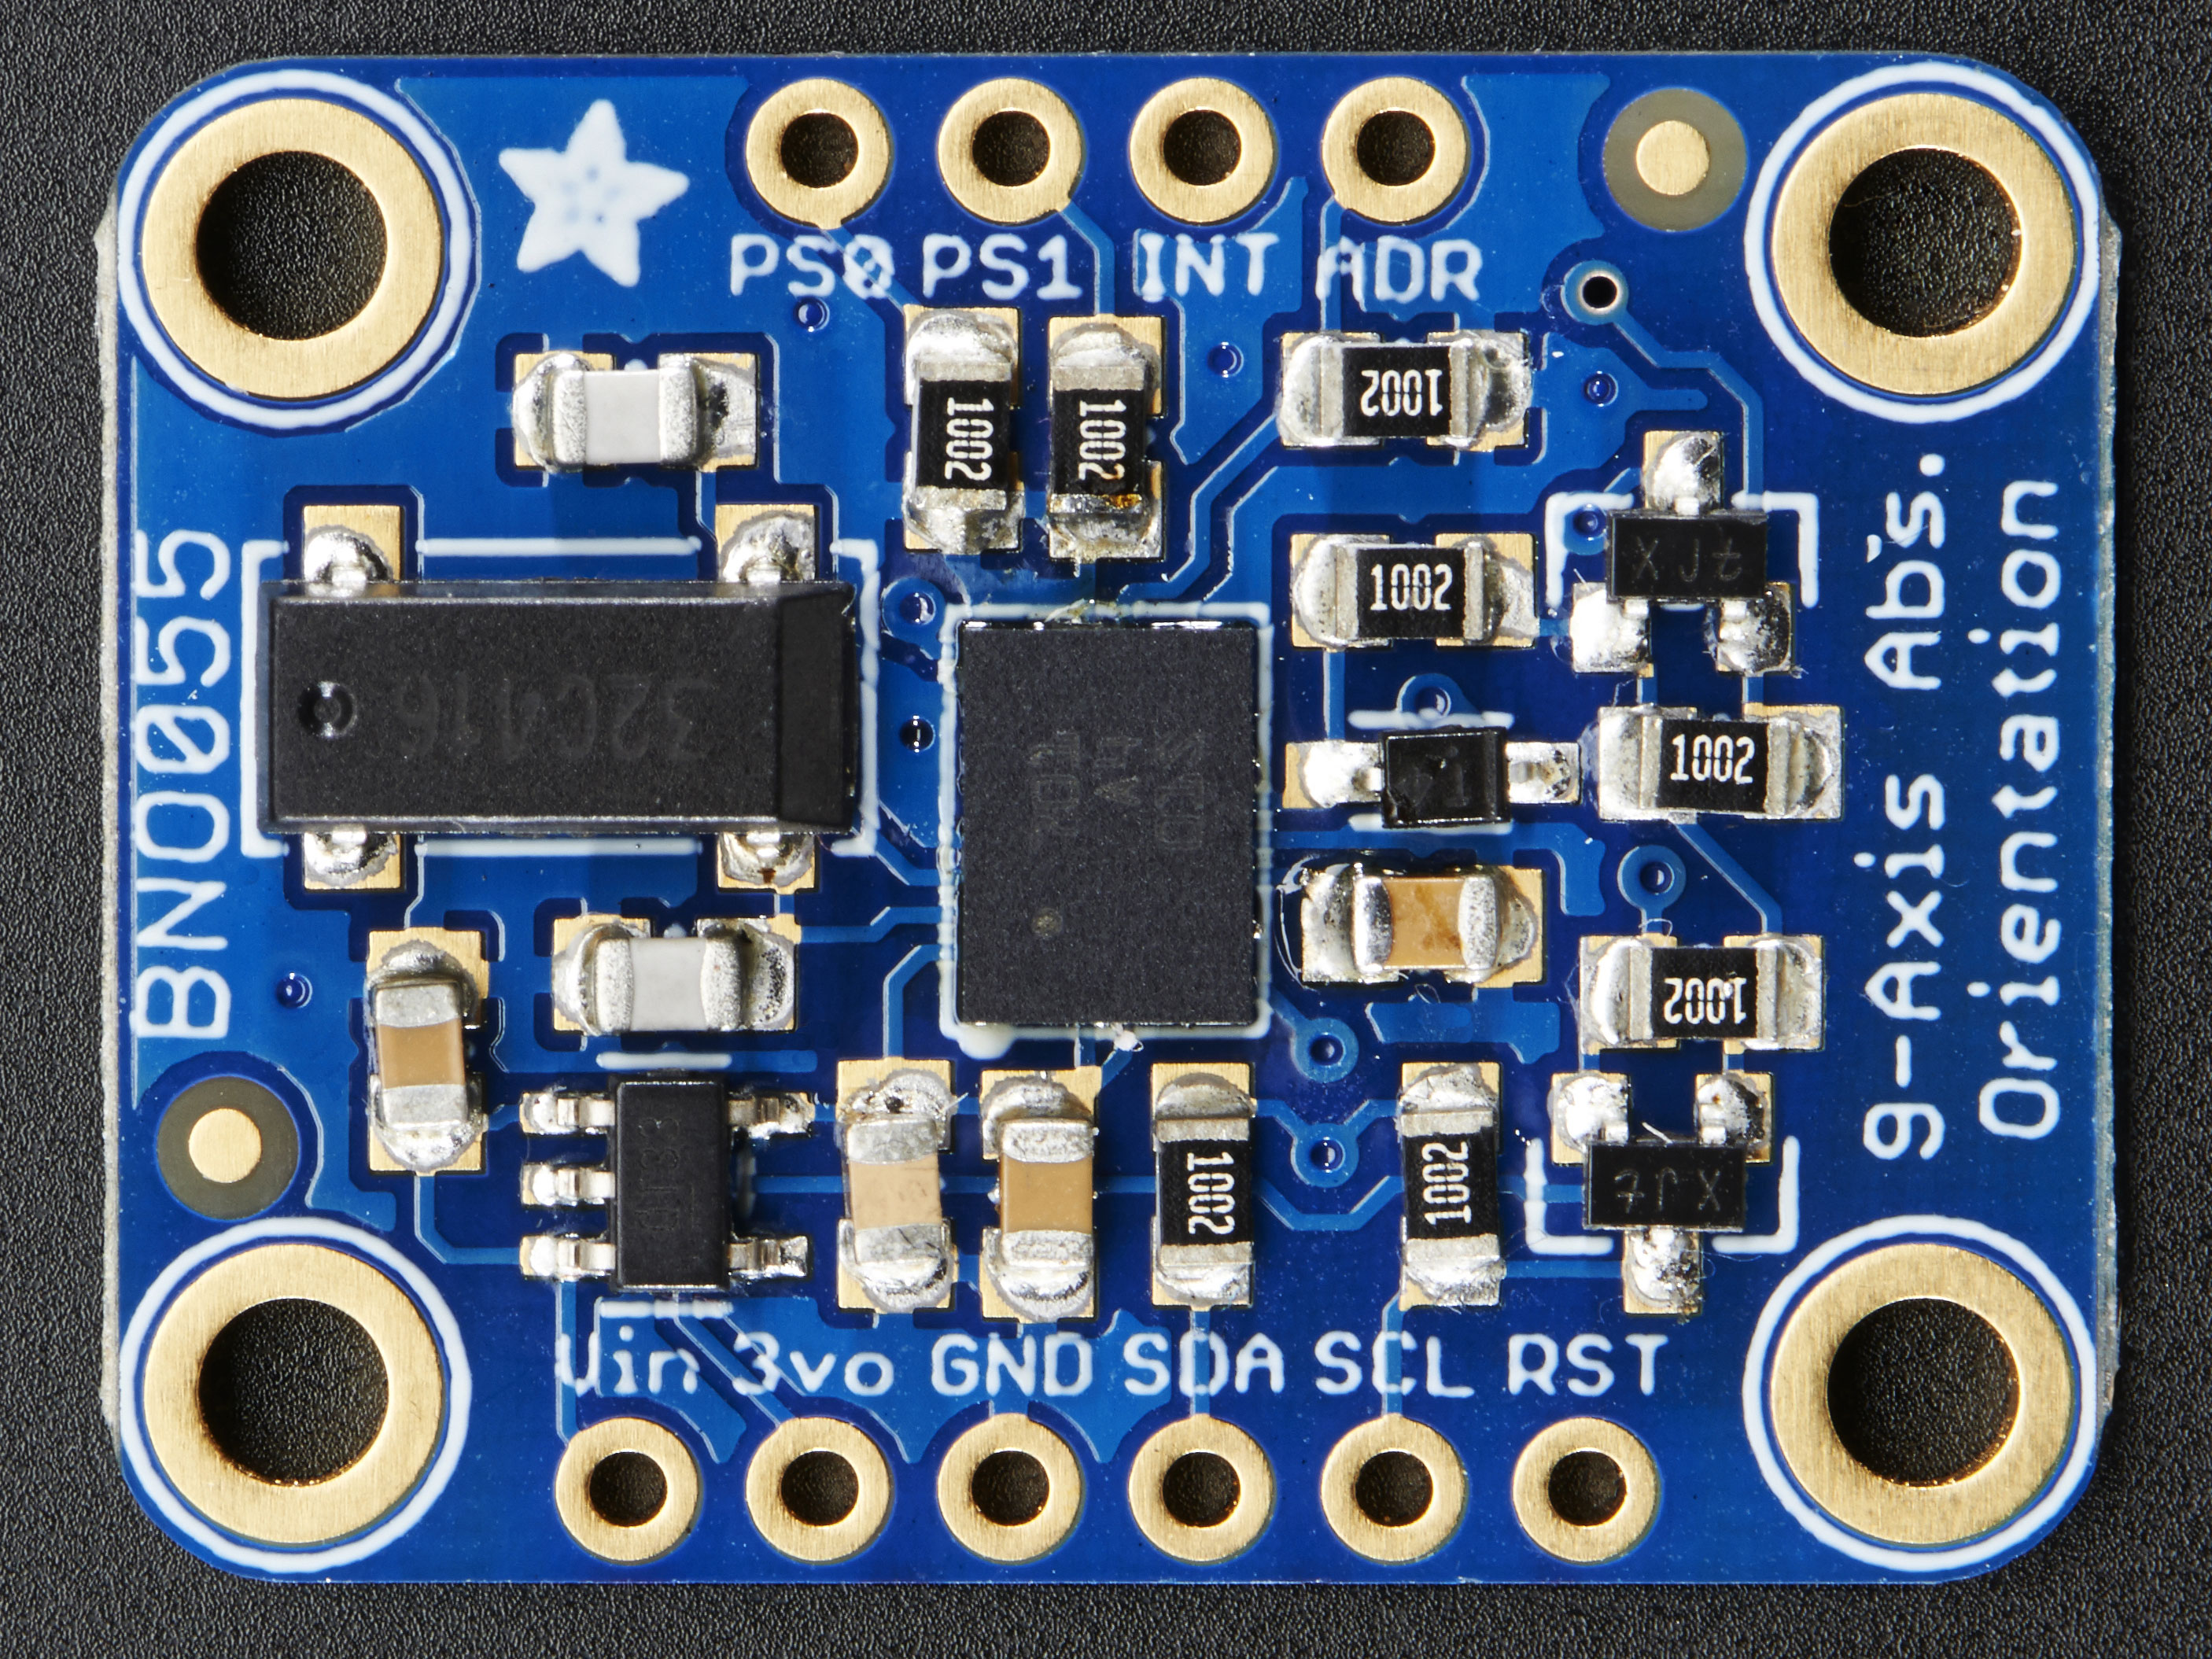
\includegraphics[width=0.5\textwidth]{src/media/hardware/bno.jpg}
\caption{Arduino BNO055 breakout board}
\label{image:bno}
\end{figure}

This (fig. \ref{image:bno}) small breakout board from Arduino has a BNO055, a 9 DOF IMU with sensor fusion on the chip. The fastest of the available protocols for data transmission on this board is I2C. Fortunately the BNO055 has an \texttt{ADR} pin, which  set to high will change its I2C address (from \texttt{0x28} to \texttt{0x29}). This allows communication with both of the used BNO055s over the same I2C bus.

Even though the RPI has pins for the I2C communication, it doesn't support clock stretching (a I2C feature used by the BNO055). Using the RPI the data collection happened at a much lower rate (around 30Hz) and generally, the connection was unreliable.

After testing different microcontrollers, the decision was made to use the Adafruit Feather HUZZAH ESP8266 board (fig. \ref{image:feather}), to read the raw data from the BNO055s and then send it directly to the RPI. Because the RPI couldn't handle reliably more than 2 BLE connections at the same time (which were already \emph{occupied} by the eSense earables), the IMU data was transmitted over the Serial Protocol (USB).

The serial payload was a string of comma separated IMU values from both BNO055, terminated with a new-line symbol: gyroscope (\texttt{x, y, z} from the \texttt{x28}), accelerometer (\texttt{x, y, z} from the \texttt{x28}), quaternion (\texttt{w, x, y, z} from the \texttt{x28}), gyroscope (\texttt{x, y, z} from the \texttt{x29}), accelerometer (\texttt{x, y, z} from the \texttt{x29}), quaternion (\texttt{w, x, y, z} from the \texttt{x29}).

When operating in the 9 DOF mode, the BNO055 needs to be calibrated every time it's powered on. To automatize this process, the BNO055s were each calibrated once, and the calibration data was stored on the Feather. Every time they were powered on, the Feather will load the calibration data first, before making any readings (see ch. \ref{subsub:feather}).

\usedspecs{Serial}{100Hz}{Accelerometer \& gyroscope \& quaternion}{Arduino BNO055 in combination with Feather Huzzah}{bno}

\begin{figure}[h!]
\centering
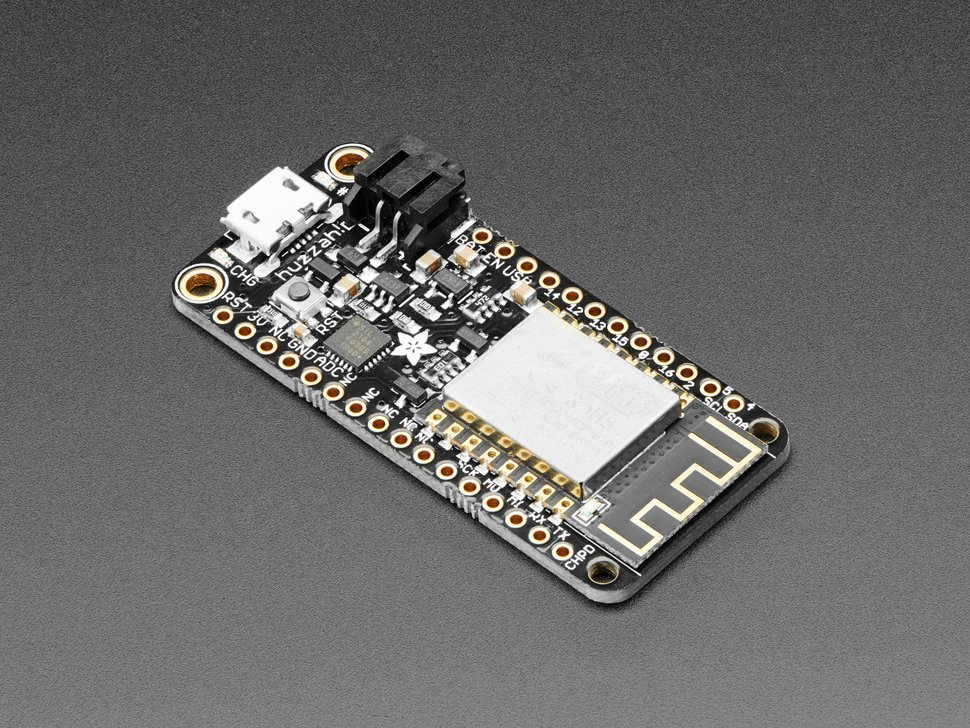
\includegraphics[width=0.5\textwidth]{src/media/hardware/feather-huzzah.jpg}
\caption{Adafruit Feather Huzzah ESP8266 board}
\label{image:feather}
\end{figure}

\begin{figure}[h!]
\centering
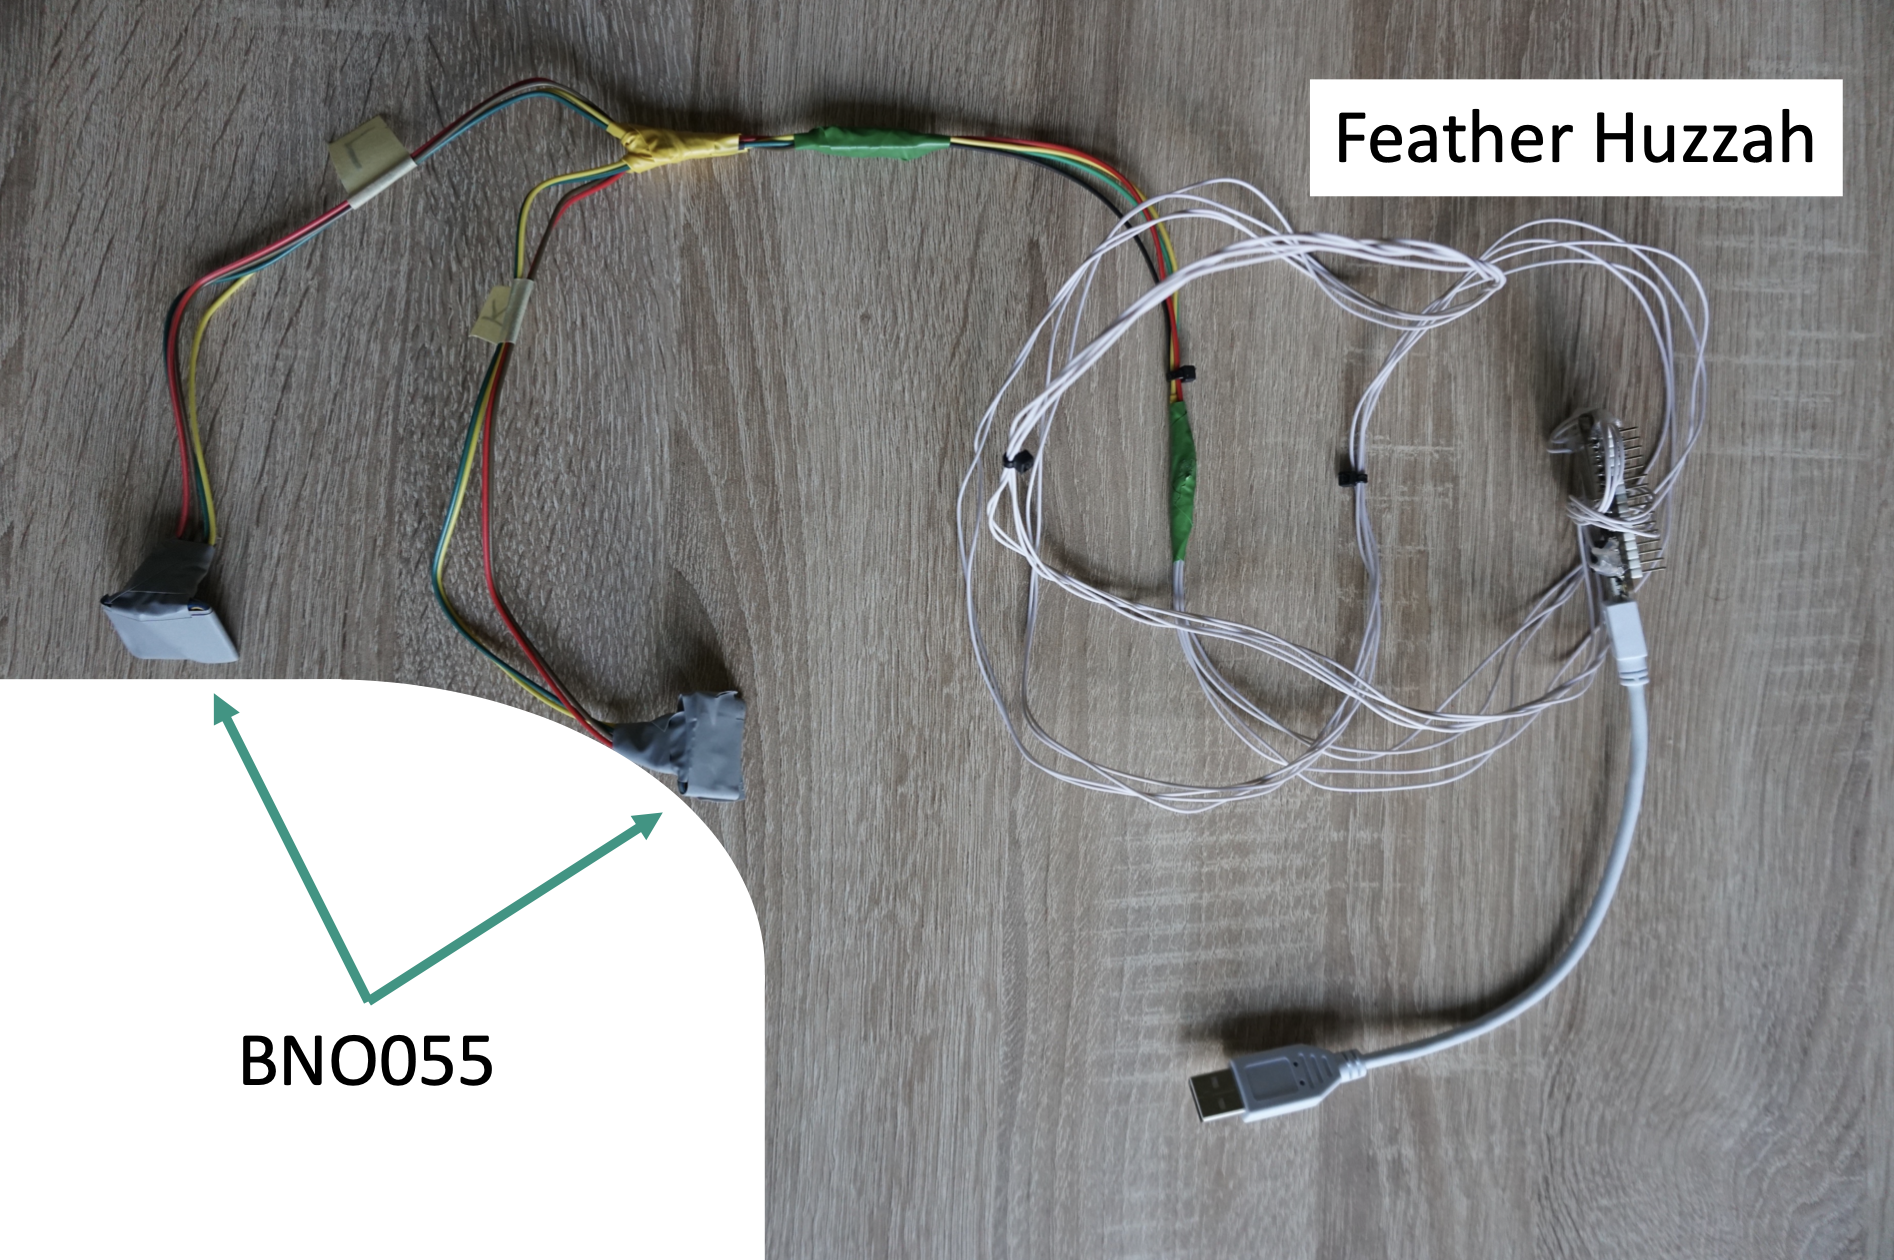
\includegraphics[width=0.8\textwidth]{src/media/hardware/real-bno.png}
\caption{Prototype of Arduino BNO055 with Feather Huzzah}
\label{image:real-bno}
\end{figure}

\subsubsection{Olimex EMG-Shield}
\label{subsub:emg}

\begin{figure}[h!]
\centering
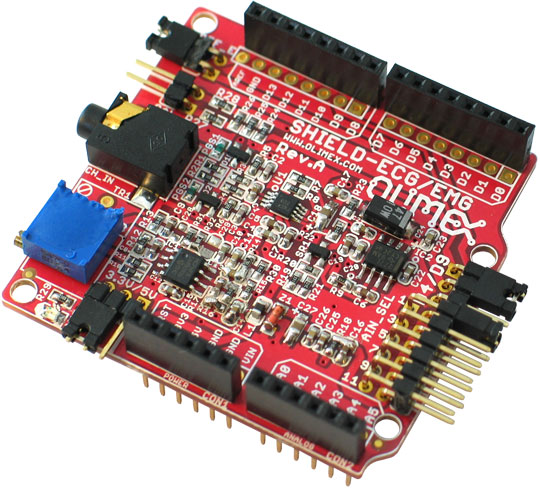
\includegraphics[width=0.5\textwidth]{src/media/hardware/emg.jpg}
\caption{Olimex EMG-Shield}
\label{image:emg}
\end{figure}

The EMG-Boards from Olimex can be stacked on top of each other, to allow readings from up to 6 channels at the same time. To capture the EMG signals from the left and right masseter muscles as well as from the left and right temporalis muscles, 4 EMG-Shields were used. The raw data from the board is analog, so an analog-to-digital (ADC) converter was needed because the RPI doesn't have any analog input pins. For this purpose, the Arduino Uno (fig. \ref{image:arduino}) was used. The collected data was sent directly to the RPI over the Serial Protocol (USB).

The serial payload consisted of 4 integer values ranging from \texttt{0} to \texttt{1023} terminated with a new-line symbol: EMG signal of the left masseter, right masseter, left temporalis, right temporalis.

\usedspecs{Serial}{256Hz}{EMG}{Olimex EMG-Shield in combination with Arduino Uno}{emg}

\begin{figure}[h!]
\centering
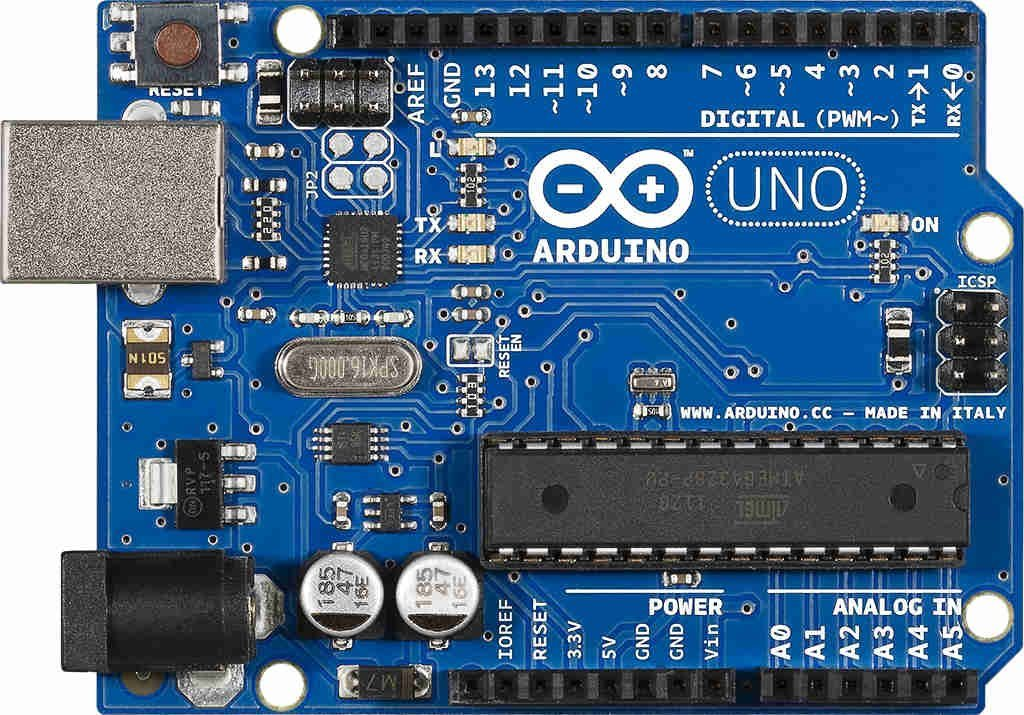
\includegraphics[width=0.5\textwidth]{src/media/hardware/arduino-uno.jpg}
\caption{Arduino Uno board}
\label{image:arduino}
\end{figure}

\begin{figure}[h!]
\centering
 \begin{subfigure}[b]{0.49\textwidth}
    \includegraphics[width=\textwidth]{src/media/hardware/real-emg-top.JPG}
    \caption{Top view}
    \label{image:real-emg-top}
  \end{subfigure}
 \hfill
 \begin{subfigure}[b]{0.49\textwidth}
    \includegraphics[width=\textwidth]{src/media/hardware/real-emg-side.JPG}
    \caption{Side view}
    \label{image:real-emg-side}
  \end{subfigure}
\caption{Prototype of EMG-Shields with Arduino Uno}
\label{image:real-emg}
\end{figure}

\subsubsection{Throat Microphone}
\label{subsub:tmic}

\begin{figure}[h!]
\centering
\includegraphics[width=0.5\textwidth]{src/media/hardware/tmic.JPG}
\caption{Throat Microphone}
\label{image:tmic}
\end{figure}

As a novelty in using wearables for bruxism detection, a throat microphone (fig. \ref{image:tmic}) was introduced to the set of peripherals. The AUX present on the RPI doesn't have the functionality to record audio. The microphone was connected directly to a laptop, which was also used to control the RPI. The raw audio data was captured with the Audacity software \cite{crook_2022}.

\usedspecs{AUX TRRS}{44.1kHz}{Raw Audio}{Throat Microphone}{tmic}

\subsubsection{Grove GSR}
\label{subsub:gsr}

\begin{figure}[h!]
\centering
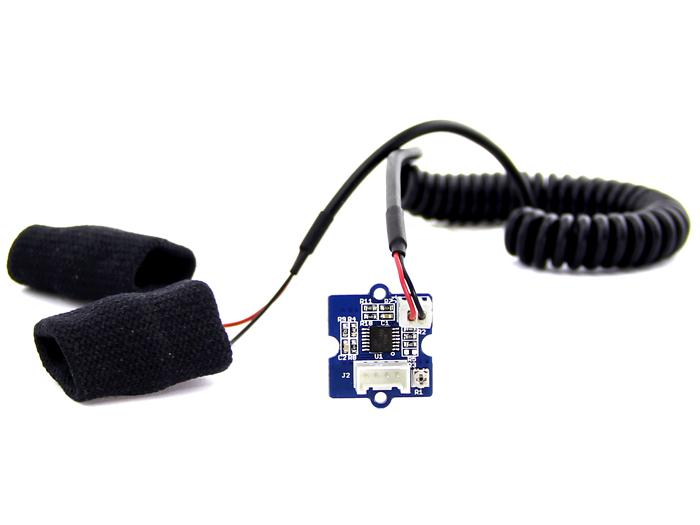
\includegraphics[width=0.5\textwidth]{src/media/hardware/gsr.jpg}
\caption{Grove GSR}
\label{image:gsr}
\end{figure}

With the Grove GSR, we can measure the electrical conductance of the skin. The raw data of this sensor is just an integer. The higher the value, the more stressed the person appears to be.

\usedspecs{Digital}{20Hz}{Galvanic skin response}{Grove GSR}{gsr}

\begin{figure}[h!]
\centering
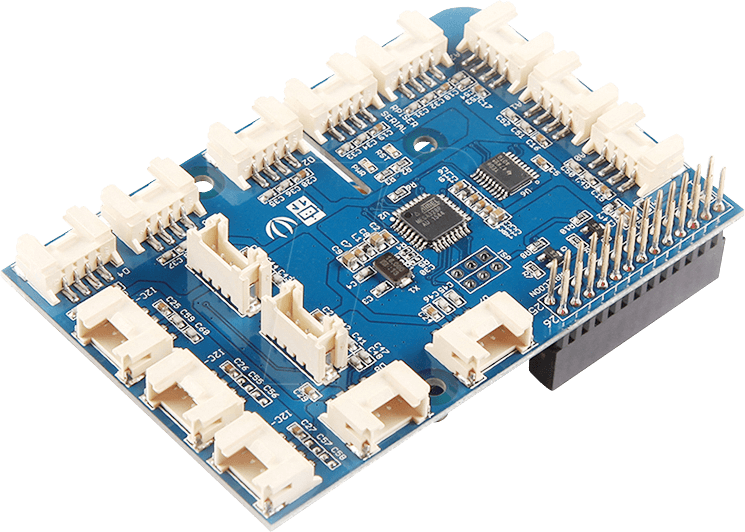
\includegraphics[width=0.5\textwidth]{src/media/hardware/grove-pi-plus.png}
\caption{Raspberry Pi Shield --- Grove Pi Plus}
\label{image:grovepi}
\end{figure}

\begin{figure}[h!]
\centering
 \begin{subfigure}[b]{0.49\textwidth}
    \includegraphics[width=\textwidth]{src/media/hardware/real-gsr-top.JPG}
    \caption{Top view}
    \label{image:real-gsr-top}
  \end{subfigure}
 \hfill
 \begin{subfigure}[b]{0.49\textwidth}
    \includegraphics[width=\textwidth]{src/media/hardware/real-gsr-side.JPG}
    \caption{Side view}
    \label{image:real-gsr-side}
  \end{subfigure}
\caption{Prototype of Grove GSR with Grove Pi Plus}
\label{image:real-gsr}
\end{figure}




\section{Software}
\label{sec:software}

To record and visualize the raw data required a custom framework with the following criteria:
\begin{itemize}
    \item \textbf{Fast}, to avoid any data loss;
    \item \textbf{Flexible}, it should be easy to add new devices, no matter what the underlying data transmission protocol is being used;
    \item \textbf{Reliable}, the captured data should be timestamped at the capture time, and be saved as soon as possible to persistent storage (par. \ref{par:data_structure}).
\end{itemize}

To sample the data at the desired rate, first, we had to ensure that the peripherals are able to send the data at \emph{that} sample rate. 

The data collection framework is implemented to be indifferent to the underlying sensor type and data transmission protocol. The yielded data was saved in a standardized format. A generic real-time data visualizer was additionally implemented.

\subsection{Microcontrollers}

\subsubsection{Feather Huzzah}
\label{subsub:feather}

As described in ch. \ref{subsub:bno}, the communication between both BNO055s and the Feather was implemented via the I2C protocol. During every user study, the BNO055 with the address \texttt{0x28} was always on the \emph{right} back side of the jaw, and the BNO055 \texttt{0x29} on the \emph{left} side accordingly.

\begin{listing}[!ht]
\begin{minted}
[
frame=lines,
framesep=2mm,
baselinestretch=1.2,
fontsize=\footnotesize,
linenos,
breaklines
]
{arduino}
#include <Wire.h>
#include <Adafruit_Sensor.h>
#include <Adafruit_BNO055.h>
#include <utility/imumaths.h>

//                                     id, address
Adafruit_BNO055 bno0 = Adafruit_BNO055(-1, 0x28);
Adafruit_BNO055 bno1 = Adafruit_BNO055(-1, 0x29);

adafruit_bno055_offsets_t bno_offset28 = { -39, -18, -39, 123, 211, -400, -1, -1, 0, 1000, 747 };
adafruit_bno055_offsets_t bno_offset29 = { -12, -28, -46, 25, 437, -66, -2, 1, 0, 1000, 718 };

sensors_event_t orientationData[2], angVelocityData[2], linearAccelData[2], magnetometerData[2], accelerometerData[2], gravityData[2];
imu::Quaternion quat[2];
\end{minted}
\caption{BBO055.ino init}
\end{listing}



On each power cycle, the devices are initialized and the calibration data is uploaded. Additionally, an external crystal (the one present on the breakout instead of the one present on the chip) is used. This increases the overall accuracy of the recorded data.

\begin{listing}[!ht]
\begin{minted}
[
frame=lines,
framesep=2mm,
baselinestretch=1.2,
fontsize=\footnotesize,
linenos
]
{arduino}
void setup(void)
{
  Serial.begin(500000);

  /* Initialise the sensor */
  setupBNO(&bno0, &bno_offset28);
  setupBNO(&bno1, &bno_offset29);
}

void setupBNO(Adafruit_BNO055* bno, adafruit_bno055_offsets_t* offsets) {
  if (!bno->begin())
  {
    /* There was a problem detecting the BNO055 ... check your connections */
    Serial.print("Ooops, no BNO055 detected ... Check your wiring or I2C ADDR!");
    while (1);
  }
  delay(1000);
  
  bno->setSensorOffsets(*offsets);
  delay(1000);

  bno->setExtCrystalUse(true);
}
\end{minted}
\caption{BBO055.ino setup}
\end{listing}


The data is then collected sequentially and sent over serial with a baudrate of 500,000. 

\begin{listing}[!ht]
\begin{minted}
[
frame=lines,
framesep=2mm,
baselinestretch=1.2,
fontsize=\footnotesize,
linenos
]
{arduino}
void loop(void)
{
  readData(&bno0, 0);
  readData(&bno1, 1);

  printData(0);
  Serial.print(",");
  printData(1);

  Serial.println();
}
\end{minted}
\caption{BBO055.ino main loop}
\end{listing}

No delays were implemented in the main loop, as it isn't possible to read the raw data from the sensors faster than the designed 100Hz.

\subsubsection{Arduino Uno}
\label{subsub:arduino}

Each of the EMG-Shields has a jumper to select the analog channel the raw data should be sent. A mapping of the analog pin to muscle was made and kept consistent through the user studies table \ref{table:emg_mapping}.

\begin{table}[!h]
\centering
\begin{tabular}{|c|c|} 
 \hline
 Analog pin & Muscle \\
 \hline\hline
 1 & Left masseter \\ 
 \hline
 2 & Right masseter \\ 
 \hline
 3 & Left temporalis \\ 
 \hline
 4 & Right temporalis \\ 
 \hline
\end{tabular}
\caption{EMG analog pin to muscle mapping}
\label{table:emg_mapping}
\end{table}

The sample rate of the EMG signals is soft-locked at 256Hz. This is the optimal operational frequency for this shield from Olimex.

\begin{listing}[!ht]
\begin{minted}
[
frame=lines,
framesep=2mm,
baselinestretch=1.2,
fontsize=\footnotesize,
linenos
]
{arduino}
// All definitions
#define NUMCHANNELS 4
#define SAMPFREQ 256                      // ADC sampling rate 256
#define PERIOD_us (1000000/(SAMPFREQ))    // Set 256Hz sampling frequency       

// Global constants and variables
unsigned char CurrentCh;         //Current channel being sampled.
unsigned long last_us = 0L;      // Helper for the sample rate
\end{minted}
\caption{EMG.ino init}
\end{listing}

The analog pins are being read sequentially and sent over serial with a baudrate of 115,200.

\begin{listing}[!ht]
\begin{minted}
[
frame=lines,
framesep=2mm,
baselinestretch=1.2,
fontsize=\footnotesize,
linenos
]
{arduino}
void setup() {
 Serial.begin(115200);
}

void loop() {
  if (micros() - last_us > PERIOD_us) {
    last_us += PERIOD_us;

    //Read the 4 ADC inputs
    for(CurrentCh = 0; CurrentCh < NUMCHANNELS; CurrentCh++){
        Serial.print(analogRead(CurrentCh)); 

      if (CurrentCh != NUMCHANNELS - 1) {
        Serial.print(","); 
      }
    }
    Serial.println();
  }
}
\end{minted}
\caption{EMG.ino setup and main loop}
\end{listing}

\subsection{Raspberry Pi}

A data collection framework (\ref{subsub:collector}) and a real-time data visualizer (\ref{subsub:visualizer}) were implemented for the RPI. Both can be deployed on any system capable of running python version 3.7. The only restriction would be the set of peripherals and the availability of the required communication protocols on the said systems. Which can still be easily adjusted if necessary. 

\subsubsection{Data Collection Framework}
\label{subsub:collector}

\paragraph{Overview}

The data collection framework is a command-line application written in python. It provides a generic interface to add new sensors, as well as the ability to create virtual sensors with a predefined sample rate. It accepts the name of the participant as the single command-line argument. 

As it runs completely on the RPI, an Ethernet cable was used to connect it over SSH. Before each user study, the script is started with a code-name generated by the participant. From this point the activity of the script can be divided into two phases:
\begin{enumerate}
    \item Sequentially, initialize every in-code defined sensor; Spawn 2 main coroutines per defined sensor (see par. \ref{par:sensor}); Spawn keyboard event listener coroutine.
    \item Run spawned coroutines concurrently until a keyboard event listener coroutine will be triggered to stop the script execution.
\end{enumerate}

The concurrency is achieved with the \texttt{asyncio} package. To be able to achieve the desired speed in data collection, all of the I/O-related tasks (as sensor readings) should be written in a non-blocking fashion. All coroutines are prepended with the \texttt{async} keyword in the signature. To signal a coroutine switch the \texttt{await} keyword is used before the call to a coroutine.

\begin{listing}[!ht]
\begin{minted}
[
frame=lines,
framesep=2mm,
baselinestretch=1.2,
fontsize=\footnotesize,
linenos
]
{python}
if __name__ == "__main__":
    logging.basicConfig(format='%(asctime)s - %(message)s',
                        datefmt='%d.%m.%Y %H:%M:%S', level=logging.INFO)

    dir_name = sys.argv[1]
    halt_event = asyncio.Event()
    asyncio.run(main(dir_name, halt_event))
\end{minted}
\caption{Data collection framework entry point}
\end{listing}

\begin{listing}[!ht]
\begin{minted}
[
frame=lines,
framesep=2mm,
baselinestretch=1.2,
fontsize=\footnotesize,
linenos
]
{python}
async def main(dir_name, halt_event):
    SENSORS = [
        # Sensor(name="mock-s0"), # --- virtual sensor definition
        BLE_eSense(name="ble-left", ble_device_name="eSense-0091"),
        BLE_eSense(name="ble-right", ble_device_name="eSense-0398"),
        GSR_Grovepi(name="gsr"),
        EMG_Olimex_x4(name="emg"),
        BNO055_x2(name="bno"),
        # ...
    ]

    device = Bruxi(dir_name=dir_name, sensors=SENSORS, halt_event=halt_event)

    logger.info(
        f"Initialising {len(device.sensors)}/ {len(SENSORS)} sensors..")
    await device.initialize_sensors()
    logger.info("Done.")

    cli_event_handler = ainput(halt_event)

    logger.info("Spawning workers..")
    await asyncio.gather(*device.spawn_coroutines(), cli_event_handler)
    logger.info("All workers exited.")
\end{minted}
\caption{Data collection framework main event loop}
\end{listing}

\paragraph{Sensor Interface}
\label{par:sensor}

The generic sensor interface implements the reactor pattern (list. \ref{list:generic_sensor}): An asynchronous producer and an asynchronous consumer is initialized for every sensor. The purpose of the producer is either

\begin{itemize}
    \item to poll the data at the predefined sample rate (i.e. the Feather with BNO055s, see \ref{subsub:bno} and \ref{subsub:feather}),
    \item or to react to incoming notifications from an external device (i.e. BLE notifications from the eSense earable, see \ref{subsub:esense}).
\end{itemize}

\begin{listing}[!ht]
\begin{minted}
[
frame=lines,
framesep=2mm,
baselinestretch=1.2,
fontsize=\footnotesize,
linenos,
breaklines
]
{python}
class Sensor:
    """Interface to ease the data collection"""

    def __init__(self, name: str, sample_rate_s: float = 0.01, csv_headers: List[str] = ["dt", "column0"]) -> None:
        self.name = name
        self.sample_rate_s = sample_rate_s
        self.producer = Producer()
        self.csv_headers = csv_headers
        self.consumer = Consumer(filename=f"{self.name}.csv", 
                queue=self.producer.queue,
                finished_execution=self.producer.finished_execution, 
                csv_headers=csv_headers)

    async def _init(self) -> None:
        """If there are methods to be awaited for the sensor initialization, add them here.
        Later you can call this method in the main loop
        """
        pass

    async def get_data(self) -> dict:
        """Override this method with proper pyshical sensor read
        """
        return {
            "dt": now(),
            "column0": 42.0
        }

    async def start_stream(self) -> None:
        """Start streaming sensor data
        Should call `self.queue(data)`
        """
        while not self.producer.finished_execution.is_set():
            # Simulate N-Hz sample rate
            if self.sample_rate_s > 0:
                await sleep(self.sample_rate_s)

            data = await self.get_data()

            await self.queue(data)

    async def queue(self, data) -> None:
        """Abstraction to produce data with the producer
        """
        await self.producer.produce(data=data)
\end{minted}
\caption{Generic Sensor interface}
\label{list:generic_sensor}
\end{listing}

The sensor producer and consumer share the same data buffer, an asynchronous queue. As the data is incoming, it is labeled with the current timestamp, and transformed in the desired \texttt{dict} structure. This payload is asynchronously put to the left side of the queue. The consumer on the other hand has an always running \texttt{while} loop, which asynchronously checks the shared queue for new payloads. If the queue is not empty, and no sensor has its data ready, the payload is removed from the right side of the queue and saved to the corresponding \texttt{.csv} file (list. \ref{list:consume_method}).

\begin{listing}[!ht]
\begin{minted}
[
frame=lines,
framesep=2mm,
baselinestretch=1.2,
fontsize=\footnotesize,
linenos,
breaklines
]
{python}
class Consumer:

    async def consume(self) -> None:
        with open(f"{self.dir}/{self.filename}", 'a') as f:
            writer = csv.writer(f)
            while not self.finished_execution.is_set():
                # wait for an item from the producer
                item = await self.queue.get()
                
                # append a new row to the .csv file
                writer.writerow(item.values())
                
                # remove the payload from the queue
                self.queue.task_done()
\end{minted}
\caption{Consumer' consume method}
\label{list:consume_method}
\end{listing}

This sensor structure is the key to having a fast and reliable data collection framework.

\paragraph{Data structure}
\label{par:data_structure}

The sensor data for every participant is saved in multiple \texttt{.csv} files in a folder named with the participant-provided code-name. The \texttt{.csv} files are named after the name of the sensor origin. The sensor names, as well as the headers for the resulted \texttt{.csv} files, are defined in-code.

\subsubsection{Data Visualizer}
\label{subsub:visualizer}

The sensors implement different communication protocols and there was no standard way of visualizing the data. Also, the visualization of multiple sensors at the same time in one single place was not possible. Using the standard output of the data collection framework (\ref{subsub:collector}), it was straightforward to connect a data visualizer, to use the development of the prototype.

\paragraph{Overview}

The real-time data visualizer consists of two main components:

\begin{enumerate}
    \item Python websocket server;
    \item Vue web application.
\end{enumerate}

\paragraph{Python Websocket Server}

Using the structure described in \ref{par:data_structure}, the websocket sever can stream the list of the code-names in the output directory on the RPI. Every such directory is a collection of \texttt{.csv} files, that can be streamed to the connected client (i.e. web browser on an external device). The most recent 100 lines from each \texttt{.csv} file are streamed at a 60Hz frequency.

\paragraph{Vue web application}

The web application is built with the Vue framework. Once connected to the websocket, the available folders will be displayed as a list of buttons. Upon clicking on a button the data stream will start (fig. \ref{image:front}).

\begin{figure}[h]
\centering
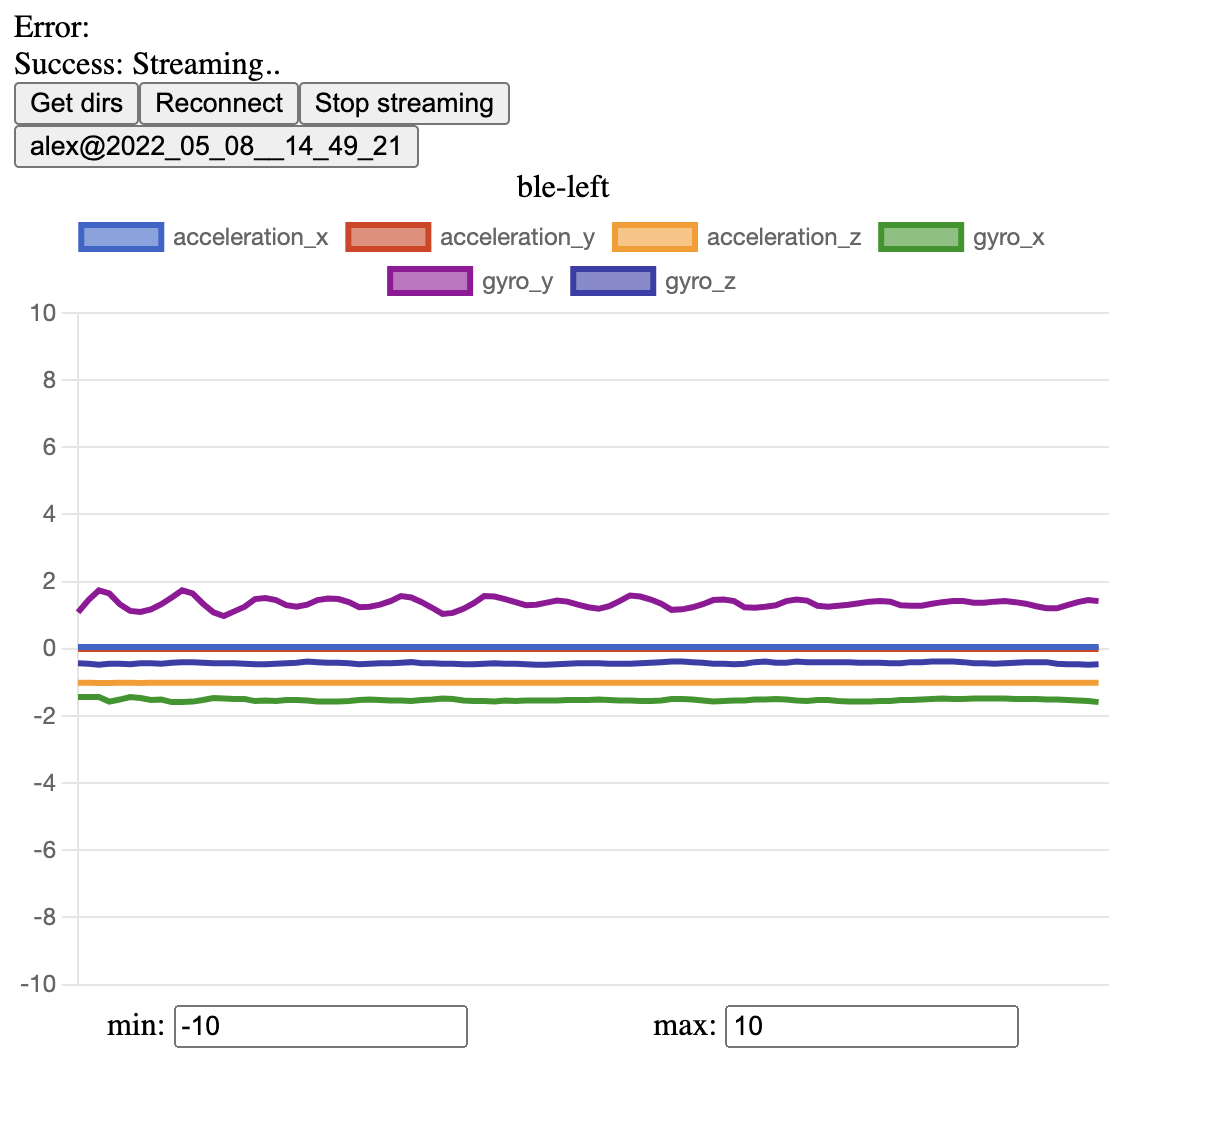
\includegraphics[width=0.8\textwidth]{src/media/software/front.png}
\caption{Vue web application example}
\label{image:front}
\end{figure}